
Para a apresentação dos resultados, é de interesse citar novamente os objetivos estabelecidos no Capítulo \ref{def_problem}. Desejávamos integrar a biblioteca OpenVDB ao Blender, de modo a permitir a visualização de volumes e dados tridimensionais salvos em arquivos desta biblioteca. No entanto, o módulo do software responsável pelos cálculos de iluminação para a exibição do resultado final está em desenvolvimento por outros desenvolvedores e ainda não é funcional.

Por isso, um artifício será utilizado na exibição dos resultados. A consulta aos valores armazenados na textura, ou seja, a amostragem dos pontos será avaliada por fatias, que, neste caso, serão planos, posicionados próximos uns aos outros, de modo a dar a impressão de visualizarmos um volume. A visualização de valores interiores ao volume será dada pelo uso de apenas um plano. Esta estratégia de visualização é exibida na Figura \ref{render_approach}.

%figura aqui!! :-P
\begin{figure}[!htb]
\center
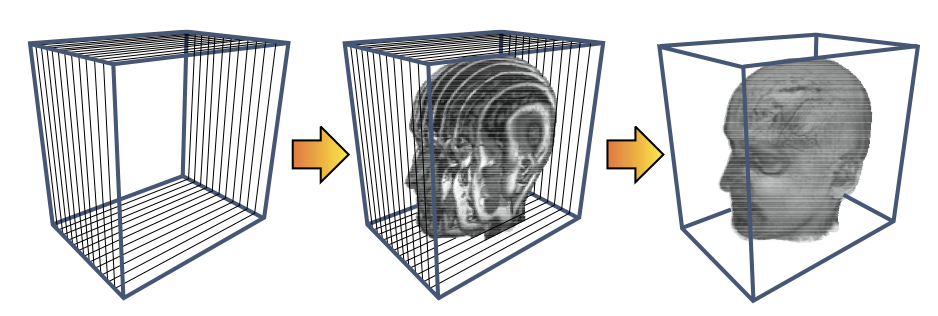
\includegraphics[width=13cm]{2drendering_approach}
\caption{À esquerda, a geometria que conterá os pontos amostrados: uma pilha de planos. No centro, a avaliação dos dados volumétricos em cada uma das fatias. À direita, o resultado da renderização, dando a impressão de visualização de um volume.}
\label{render_approach}
\end{figure}

O volume utilizado para exemplificar o funcionamento da biblioteca no Blender é exibido na Figura \ref{fig:vdb_view1}, e um corte transversal, para visualizarmos seus dados internos, é exibido nas Figuras \ref{fig:vdb_view2} e \ref{fig:vdb_view3}.

\begin{figure}[H]
        \centering
        \begin{subfigure}{0.3\textwidth}
                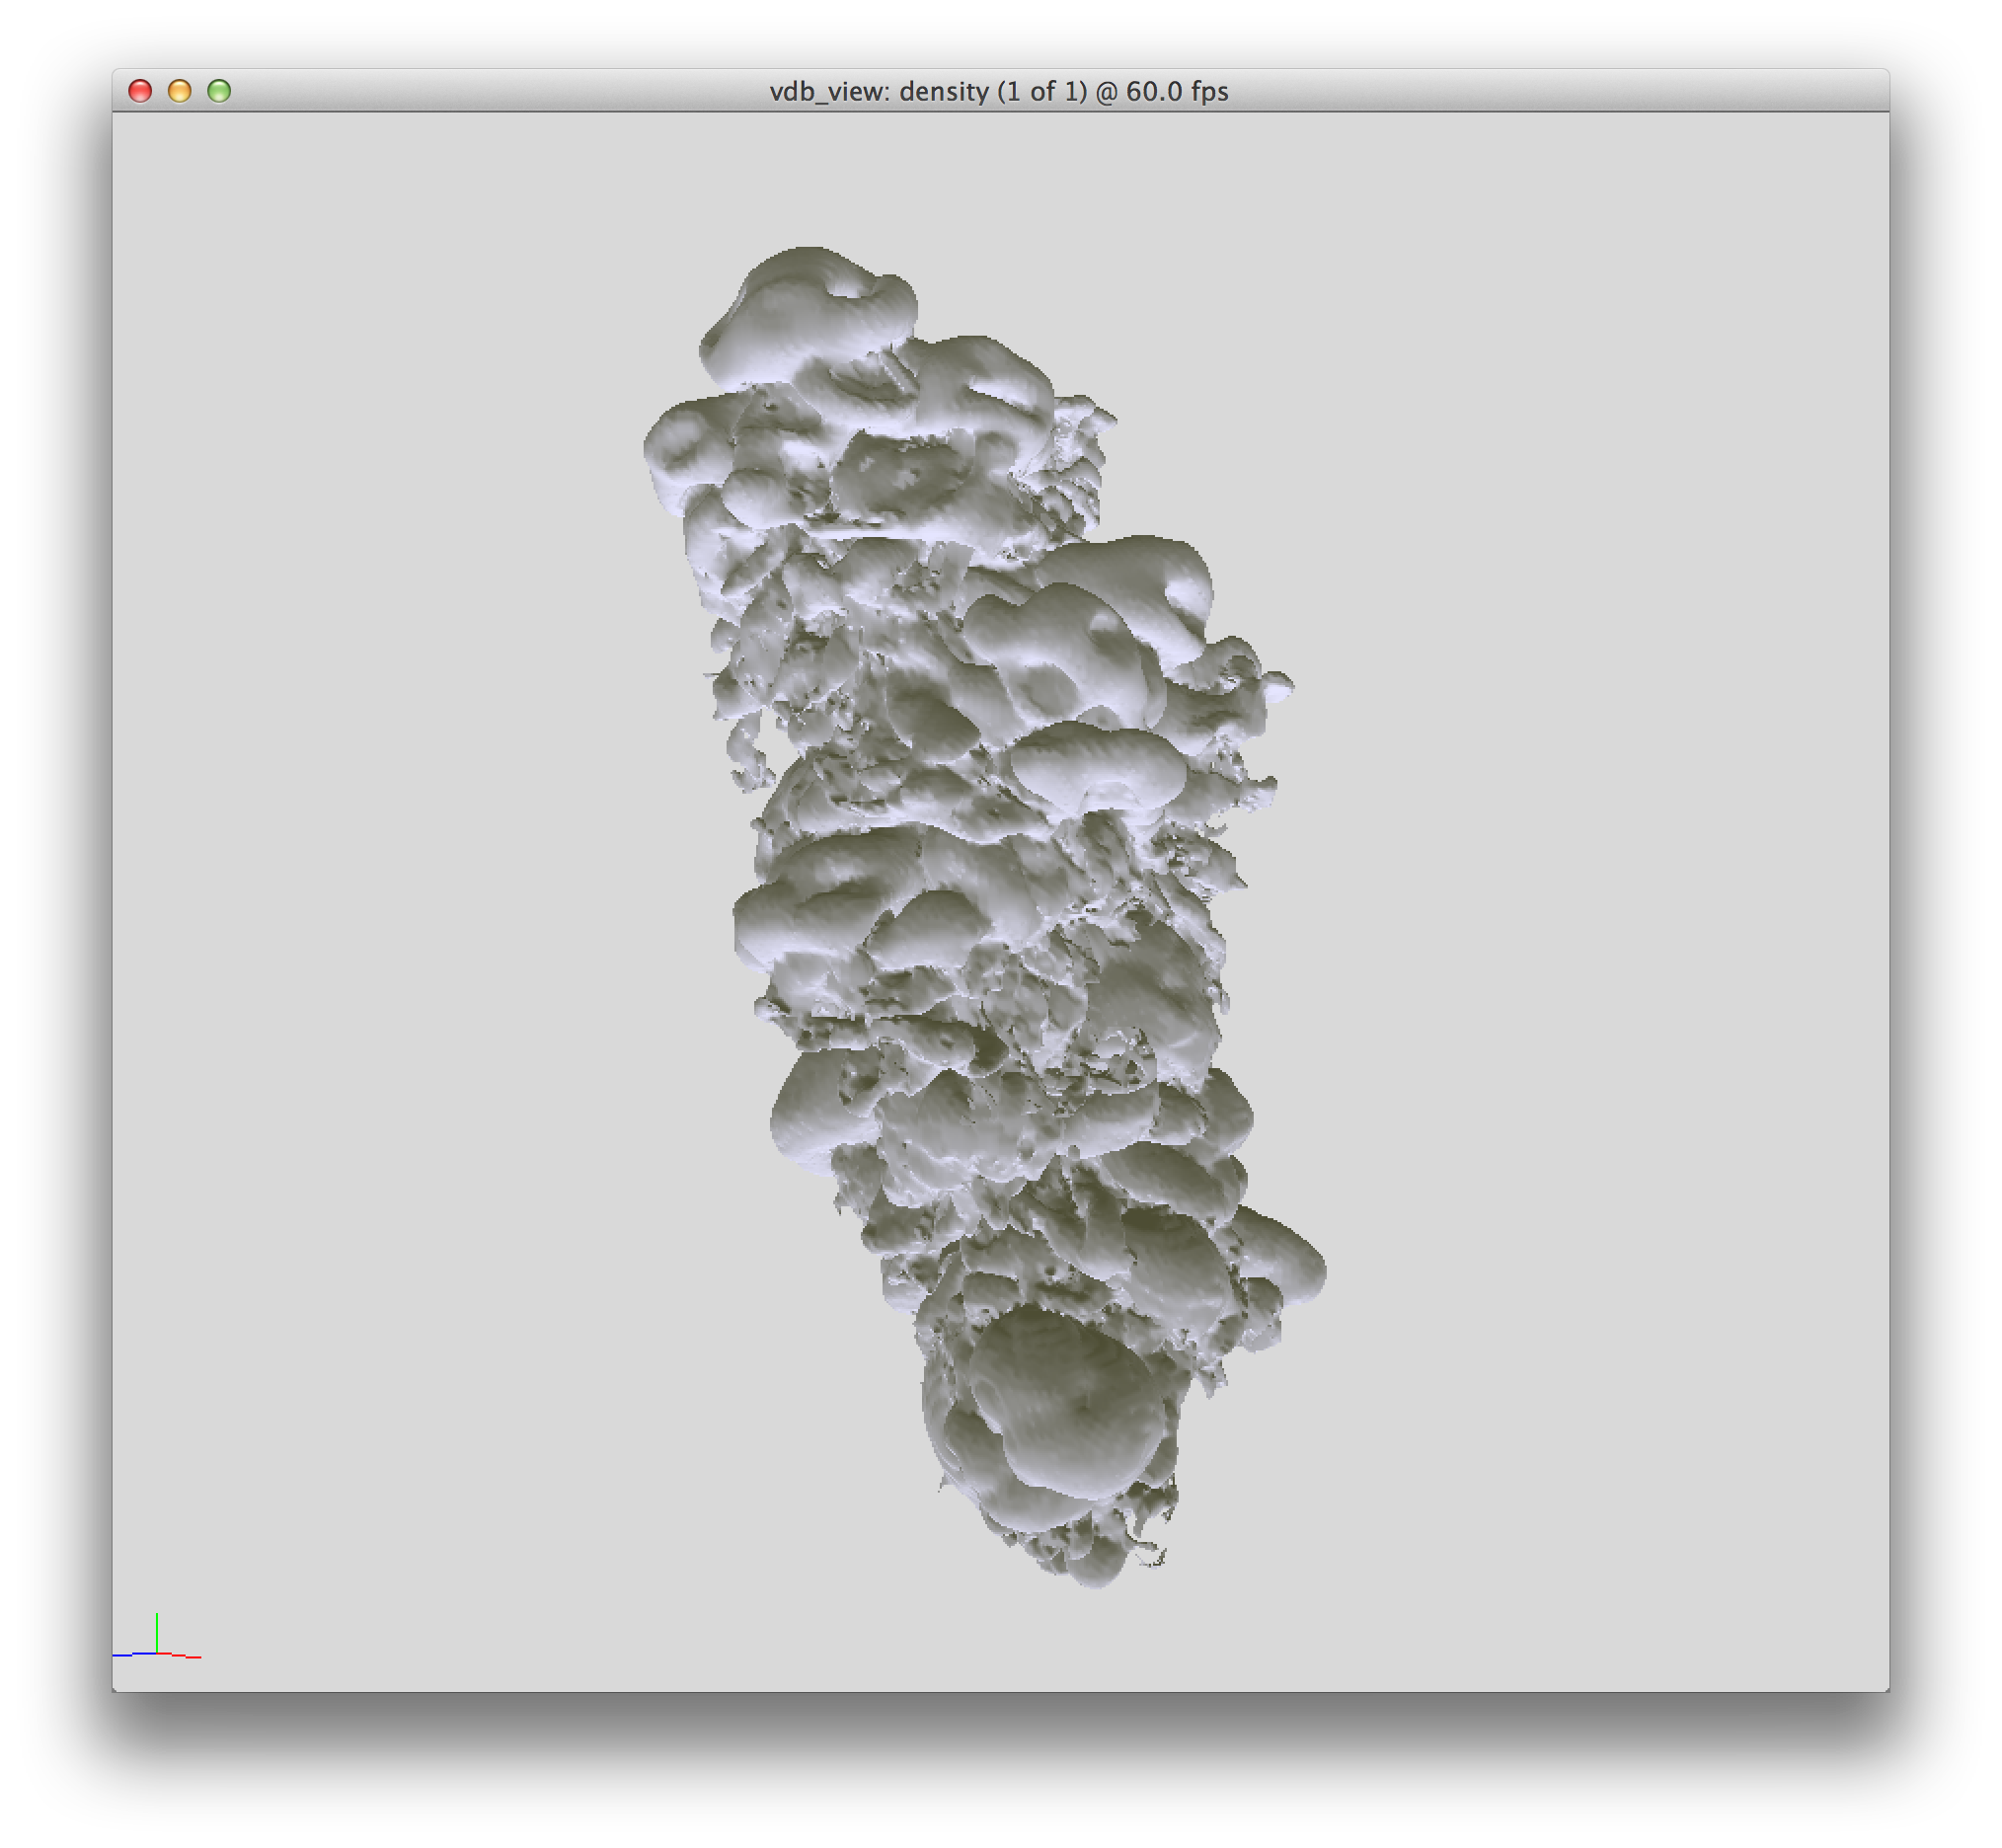
\includegraphics[width=\textwidth]{vdb_view1}
                \caption{Visão externa.}
                \label{fig:vdb_view1}
        \end{subfigure}%
        ~ %add desired spacing between images, e. g. ~, \quad, \qquad etc.
          %(or a blank line to force the subfigure onto a new line)
        \begin{subfigure}{0.3\textwidth}
                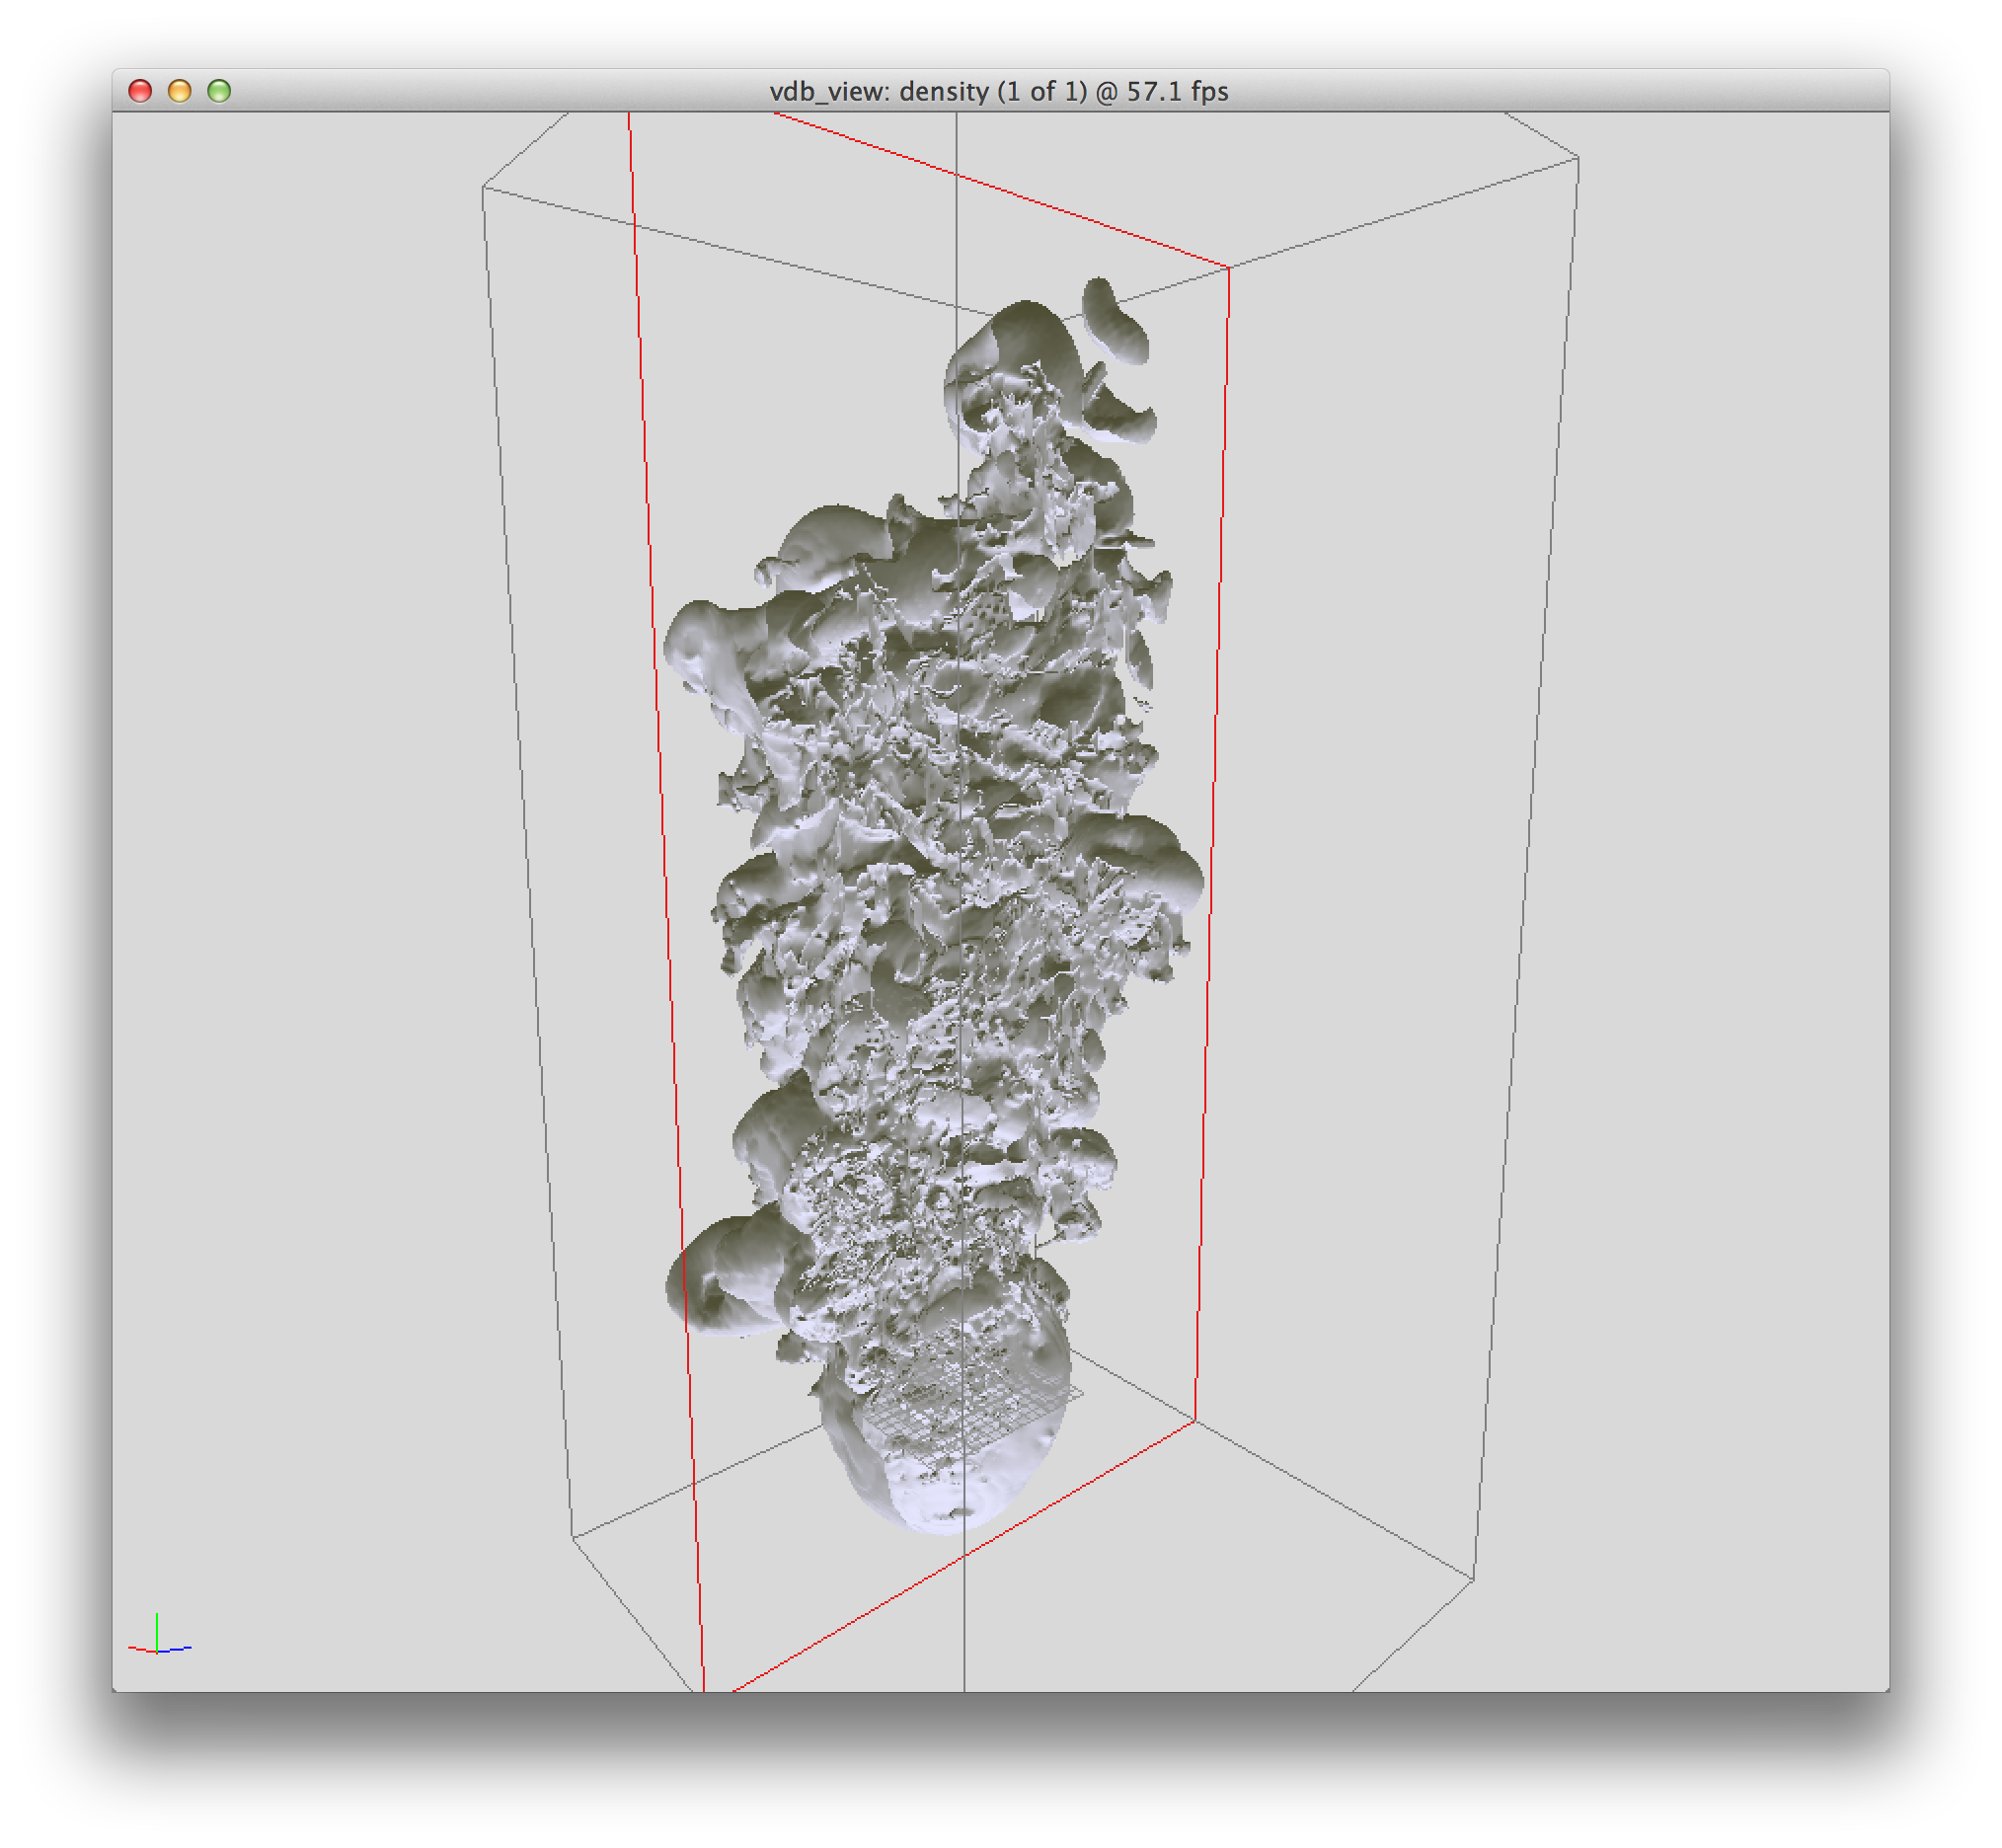
\includegraphics[width=\textwidth]{vdb_view2}
                \caption{Visão interna.}
                \label{fig:vdb_view2}
        \end{subfigure}
        ~ %add desired spacing between images, e. g. ~, \quad, \qquad etc.
          %(or a blank line to force the subfigure onto a new line)
        \begin{subfigure}{0.3\textwidth}
                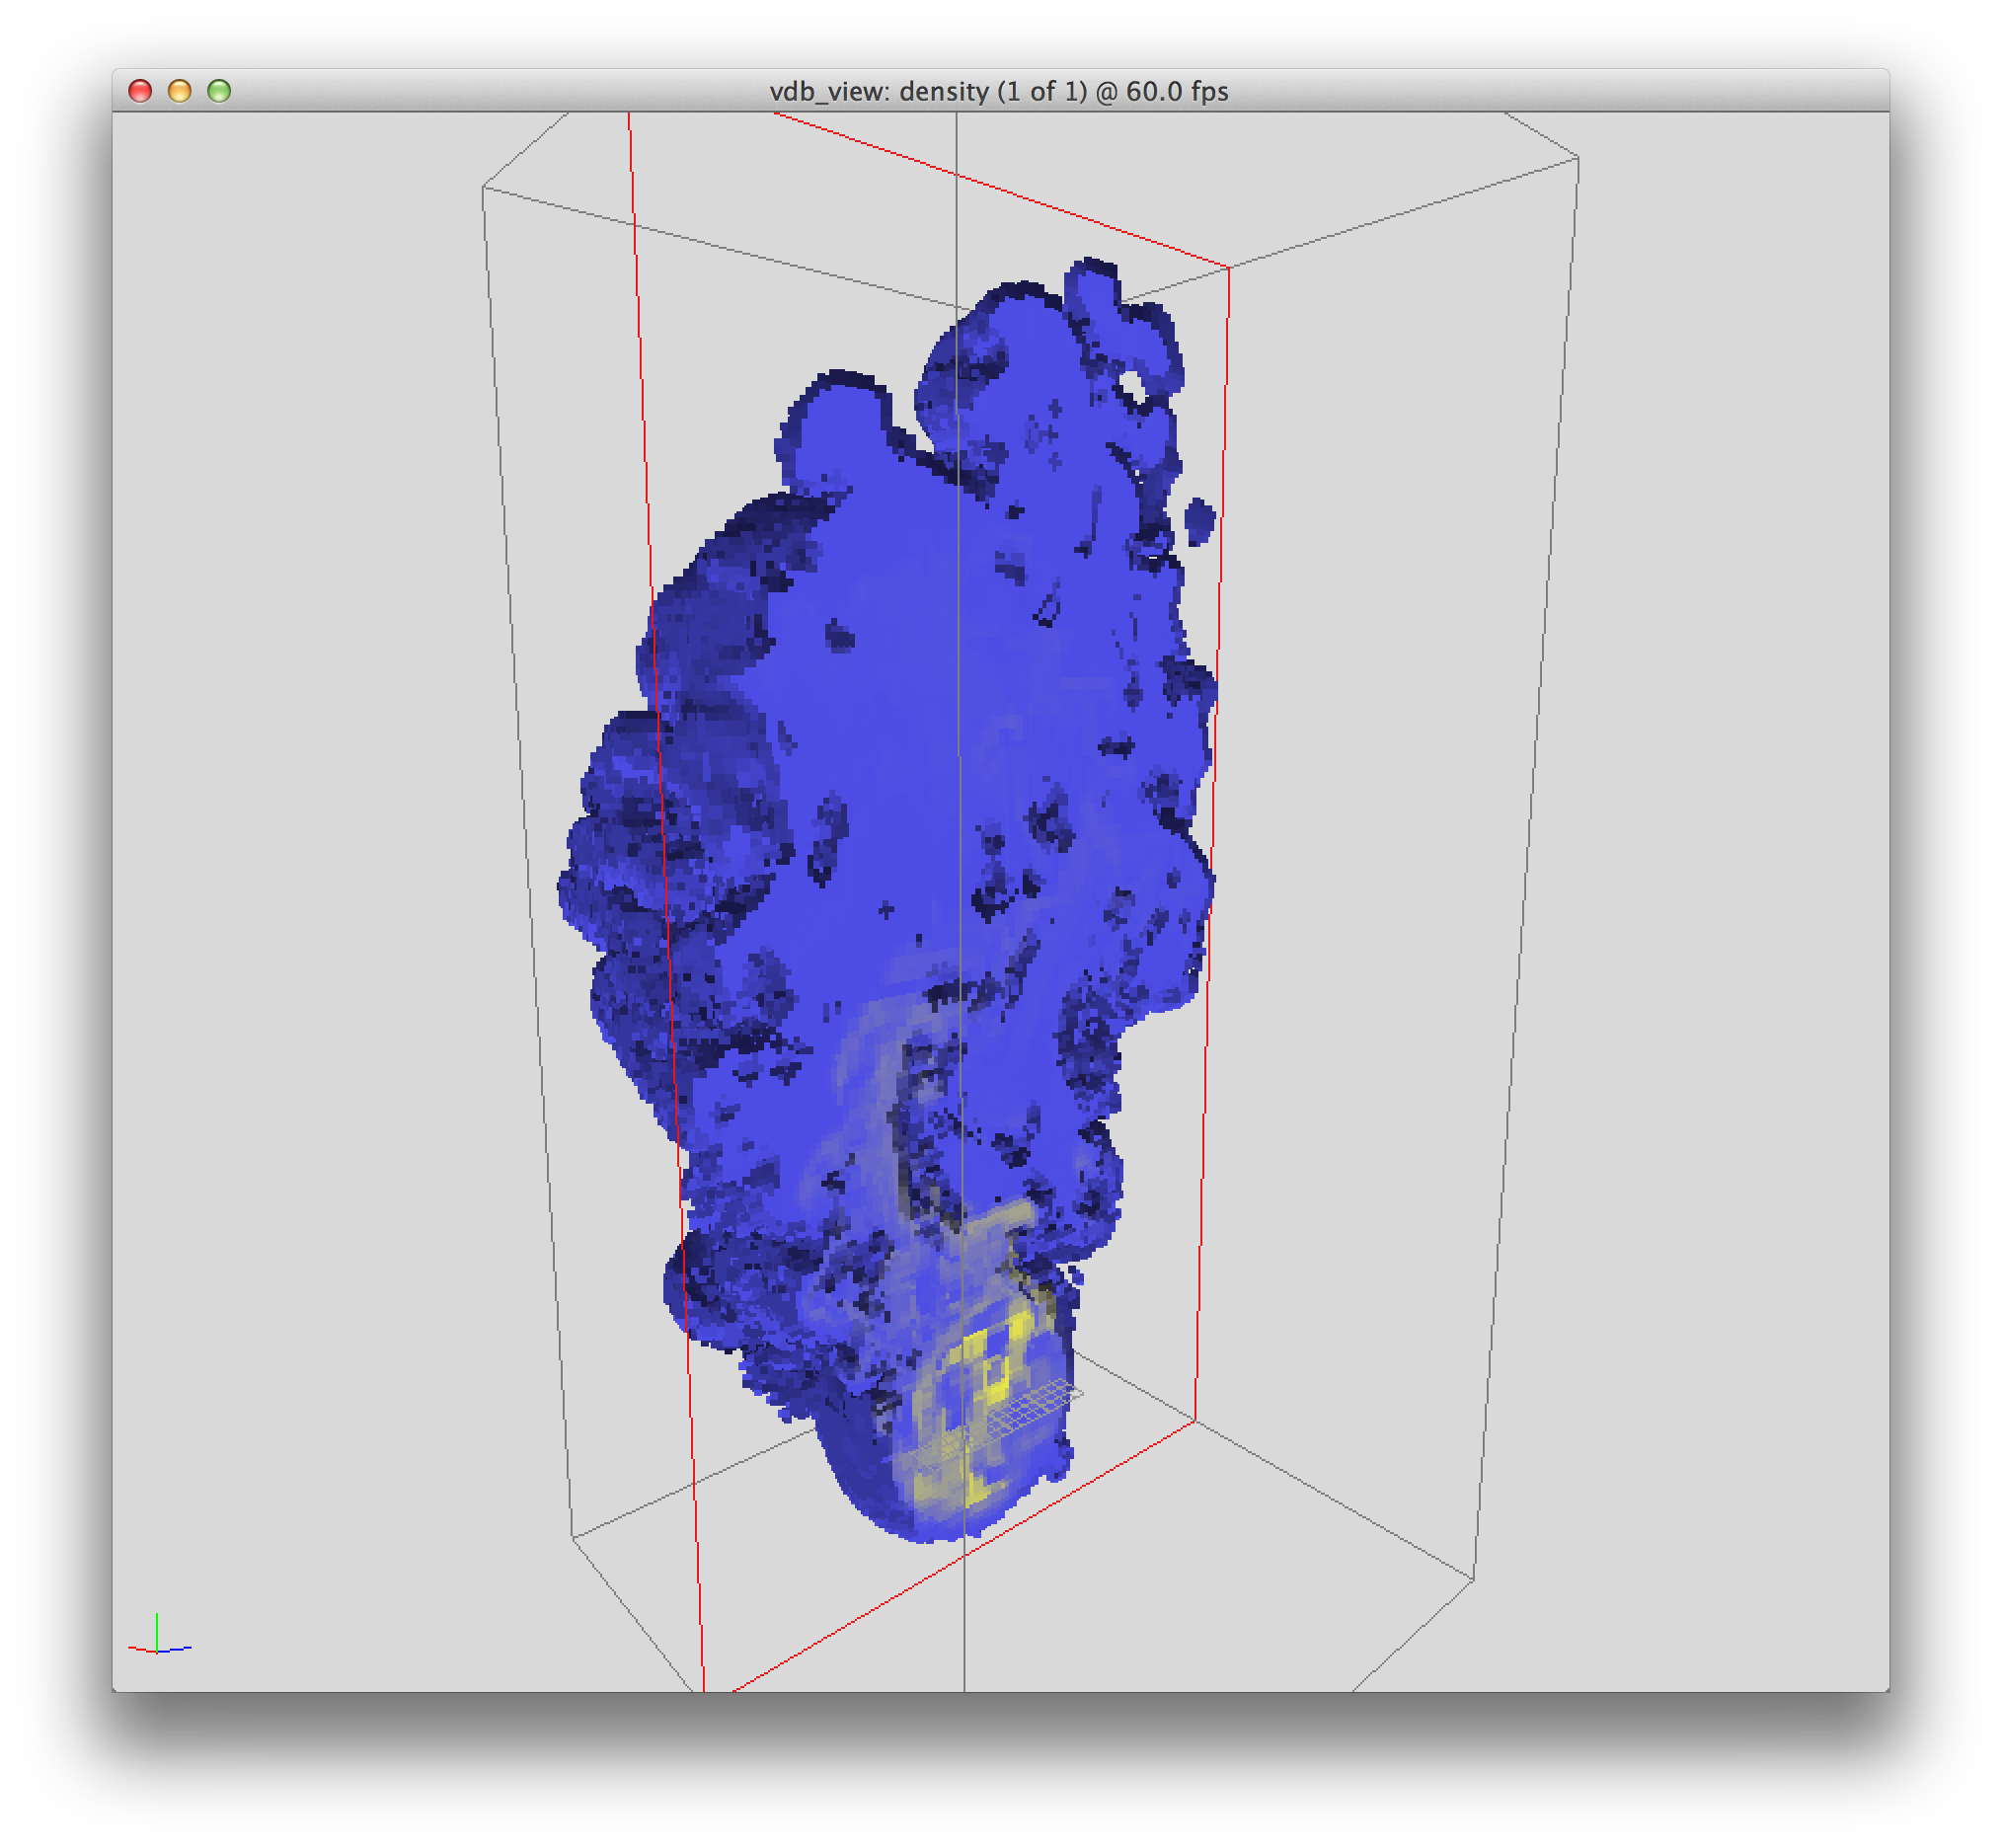
\includegraphics[width=\textwidth]{vdb_view3}
                \caption{Valores, por cor.}
                \label{fig:vdb_view3}
        \end{subfigure}
        \caption{Volume representando a densidade de uma fumaça, usada no exemplo apresentado, exibido por um visualizador específico para o formato VDB.}\label{fig:vdb_view}
\end{figure}


No Blender, o arquivo de exemplo, \texttt{smoke.vdb}, é carregado através de um nó implementado em Open Shading Language, exibido na Figura \ref{vdb_node}. E na Figura \ref{vdb_blender_interface}, a interface do Blender com a pré-visualização do mesmo volume mostrado na Figura \ref{fig:vdb_view} é exibido. As cores de exibição, que estão diferentes entre as representações, é facilmente configurável no Blender, se desejado. No Código \ref{log} é mostrada a mensagem escrita em {\it log}, com detalhes do volume carregado. Estes detalhes são obtidos a partir de \emph{metadados} salvos no arquivo e a partir de análise rápida do próprio volume. Na mensagem, a sigla \emph{bbox} refere-se ao \emph{bounding box} do volume, isto é, o menor paralelepípedo alinhado com os eixos do sistema de coordenadas que contém todo o volume. Analogamente, o termo \emph{roi} refere-se à região de interesse, na sigla em inglês. O número de \voxels e o consumo de memória em {\it bytes} também é apresentado. \\

Na Figura \ref{fig:vdb_trans}, são apresentados exemplos de aplicação de \emph{wrapping}, com operações de espelhamento em relação aos eixos y (Figura \ref{fig:vdb_trans2}) e z (Figura \ref{fig:vdb_trans3}). E finalmente, na Figura \ref{planes}, um pequeno número de planos é posicionada na cena, a uma pequena distância uns dos outros, e a textura 3D é então avaliada em cada fatia. A medida que aumentarmos o número de planos, melhor será a impressão de visualizarmos um volume.

\lstinputlisting[label=log,caption=Mensagem exibida em {\it log} quando um arquivo é carregado com sucesso.]{sourceCode/log.cpp}

%figura aqui!! :-P
\begin{figure}[!htb]
\center
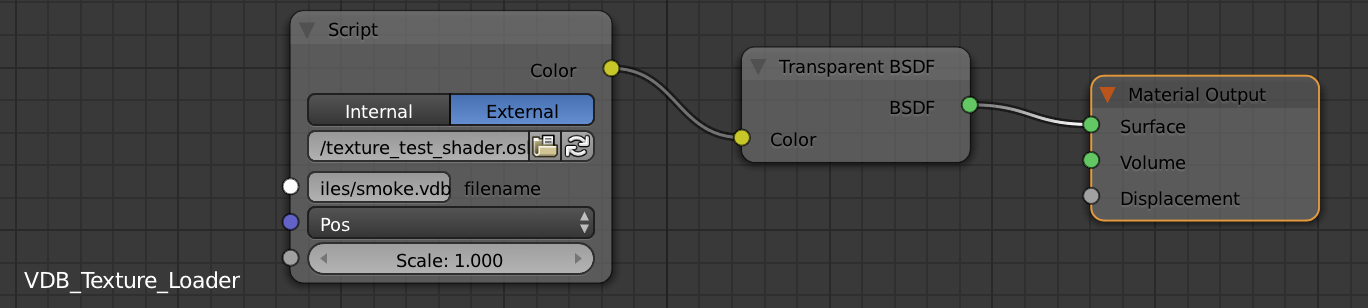
\includegraphics[width=12cm]{vdb_node}
\caption{Nó gerado a partir de código OSL especificamente para carregar arquivos VDB.}
\label{vdb_node}
\end{figure}

%figura aqui!! :-P
\begin{figure}[!htb]
\center
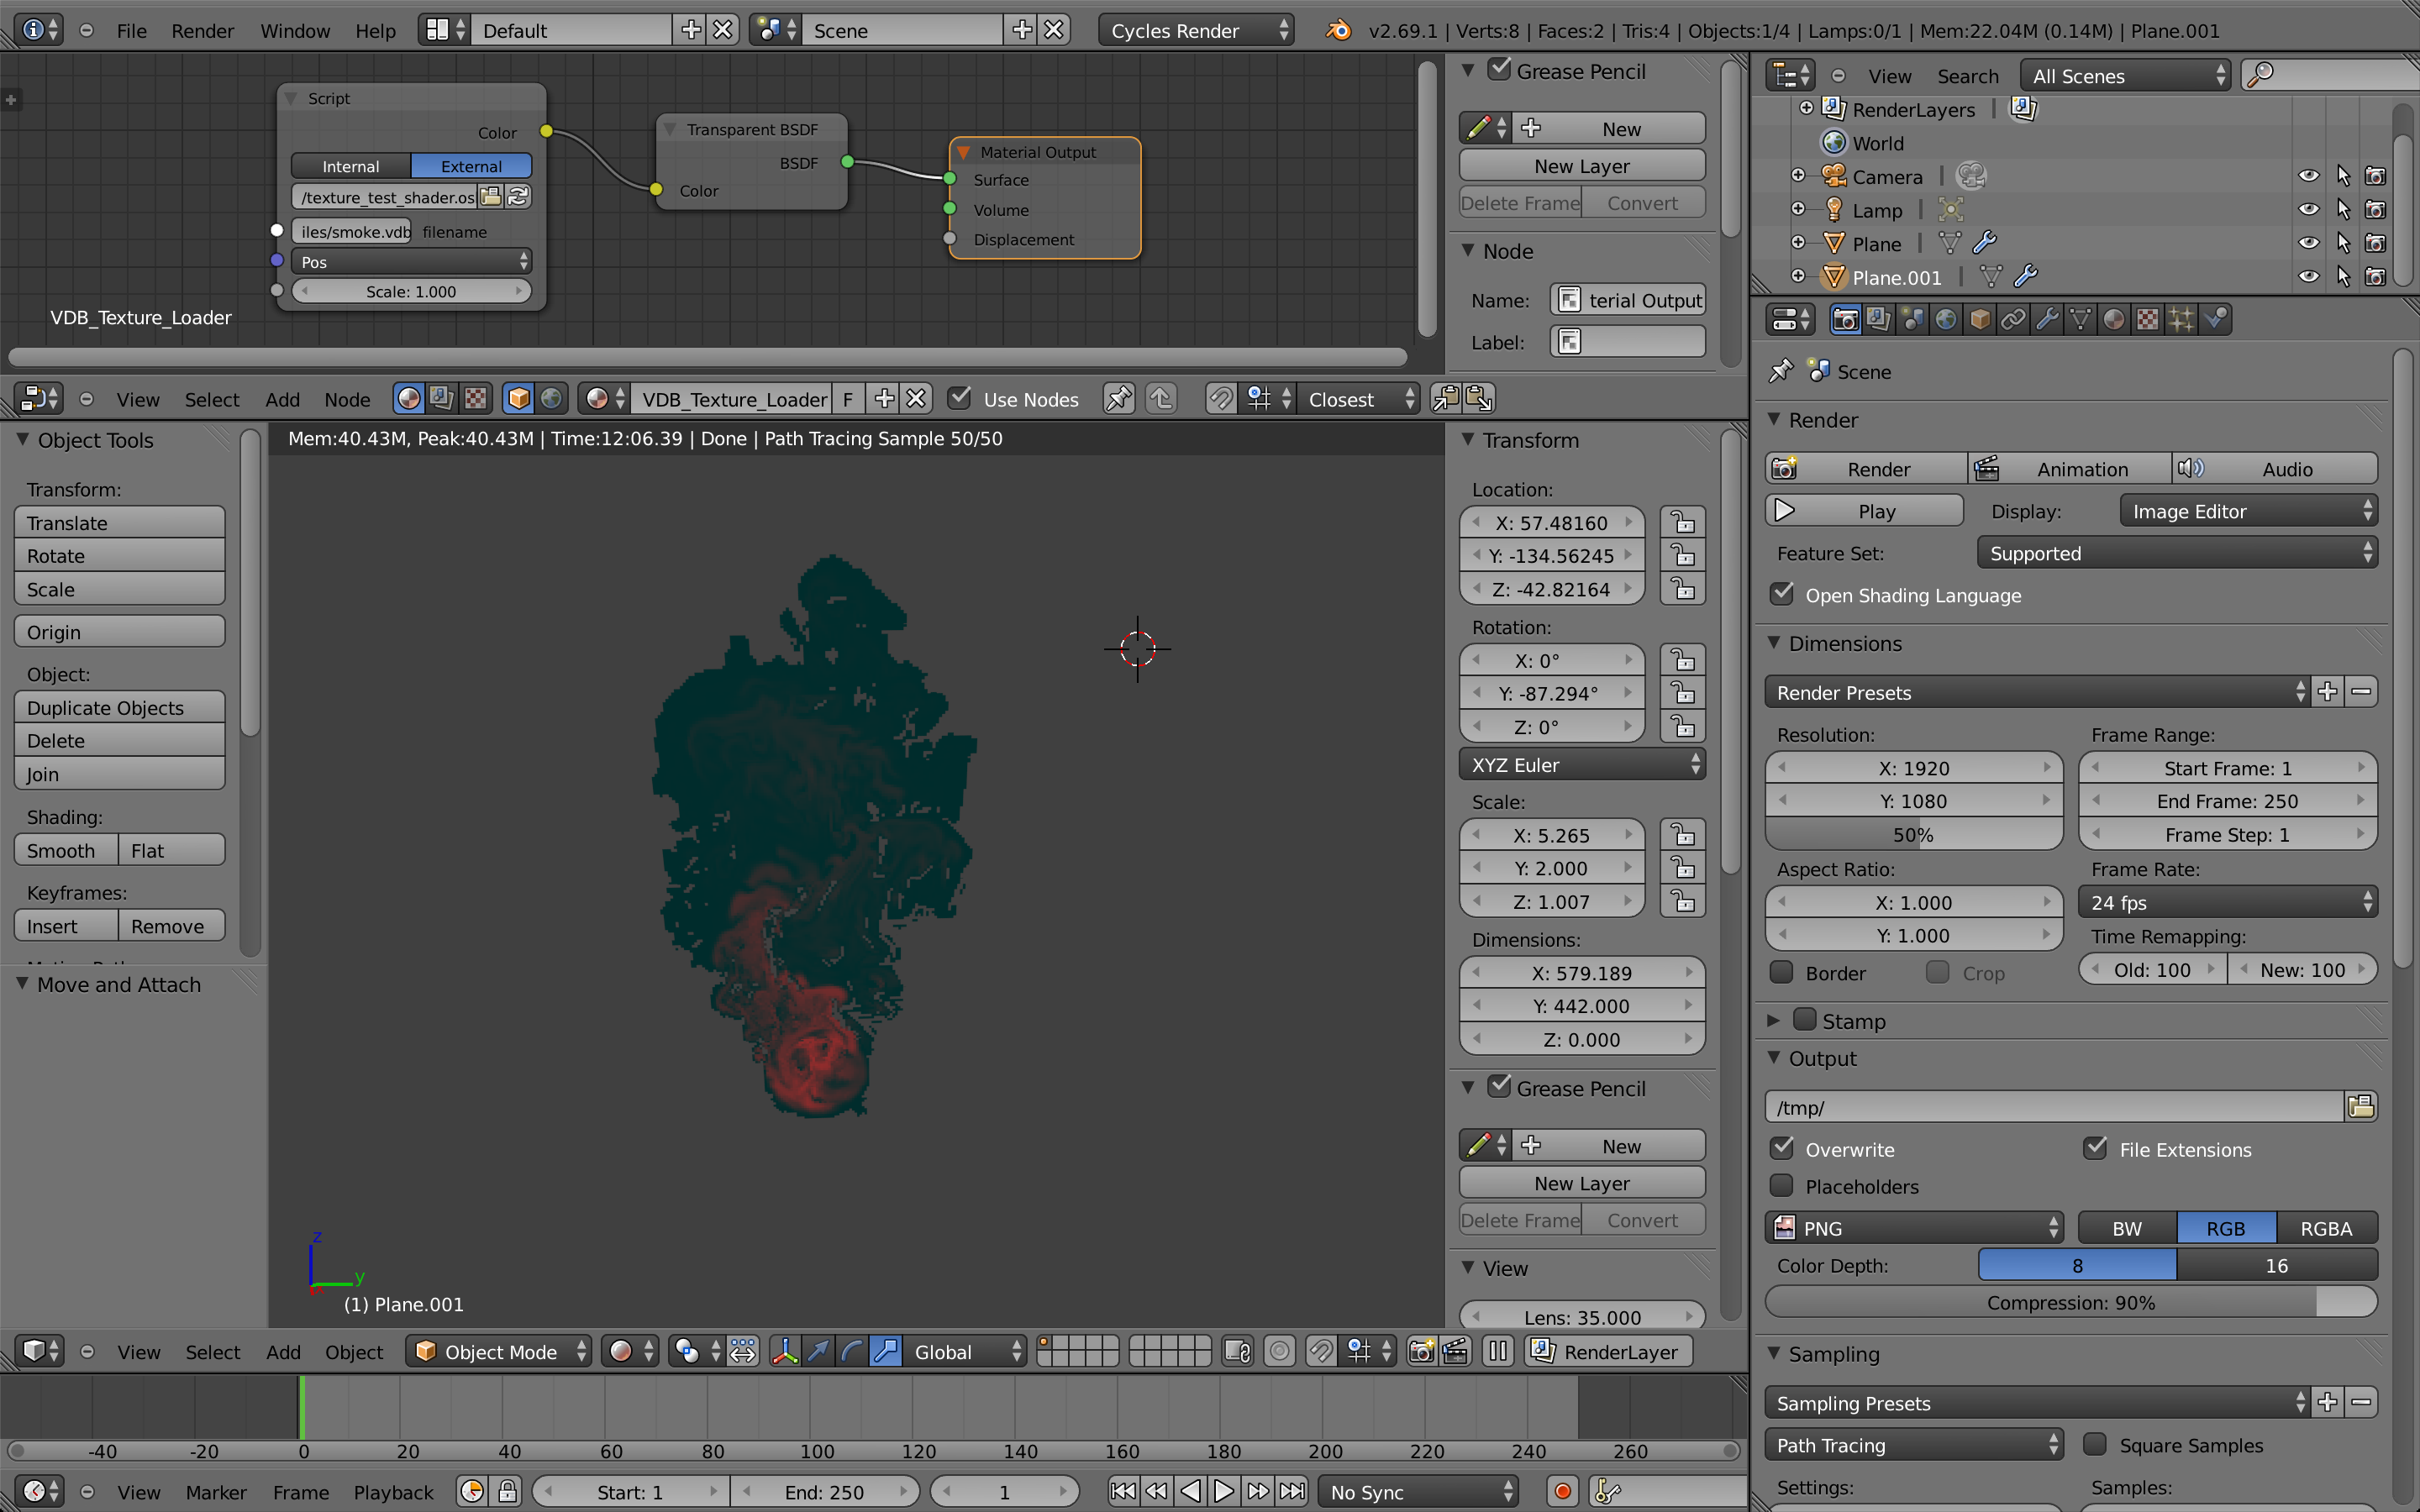
\includegraphics[width=12cm]{vdb_blender_interface}
\caption{Interface do Blender com a pré-visualização de uma fatia do volume.}
\label{vdb_blender_interface}
\end{figure}

\begin{figure}[!htb]
        \centering
        \begin{subfigure}{0.3\textwidth}
                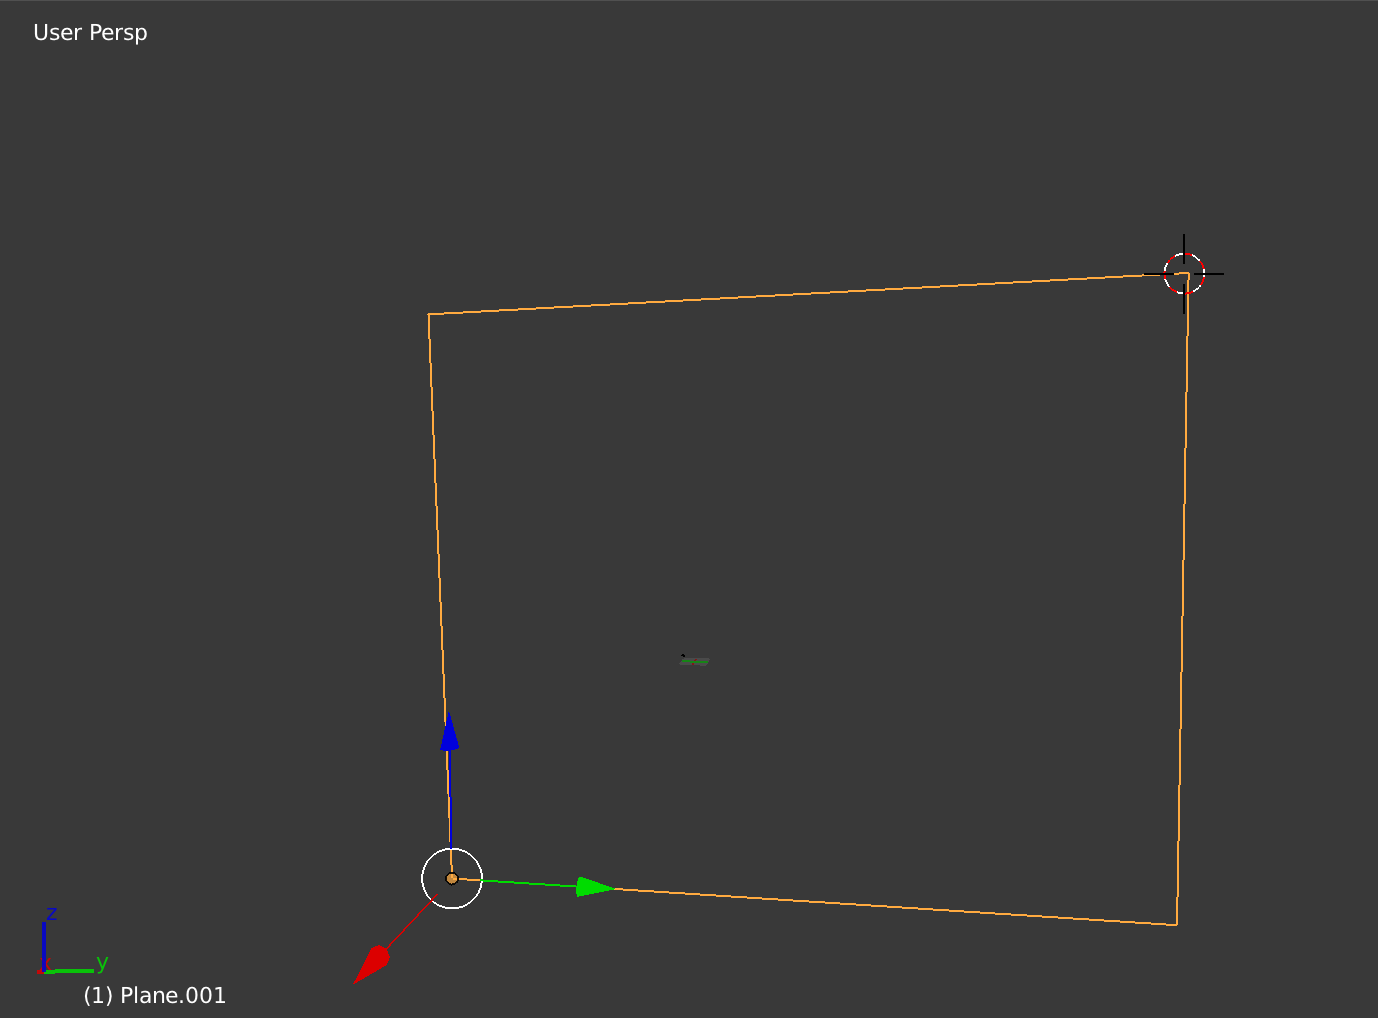
\includegraphics[width=\textwidth]{transf_geometry}
                \caption{Geometria que recebe a textura.}
                \label{fig:vdb_trans1}
        \end{subfigure}%
        ~ %add desired spacing between images, e. g. ~, \quad, \qquad etc.
          %(or a blank line to force the subfigure onto a new line)
        \begin{subfigure}{0.3\textwidth}
                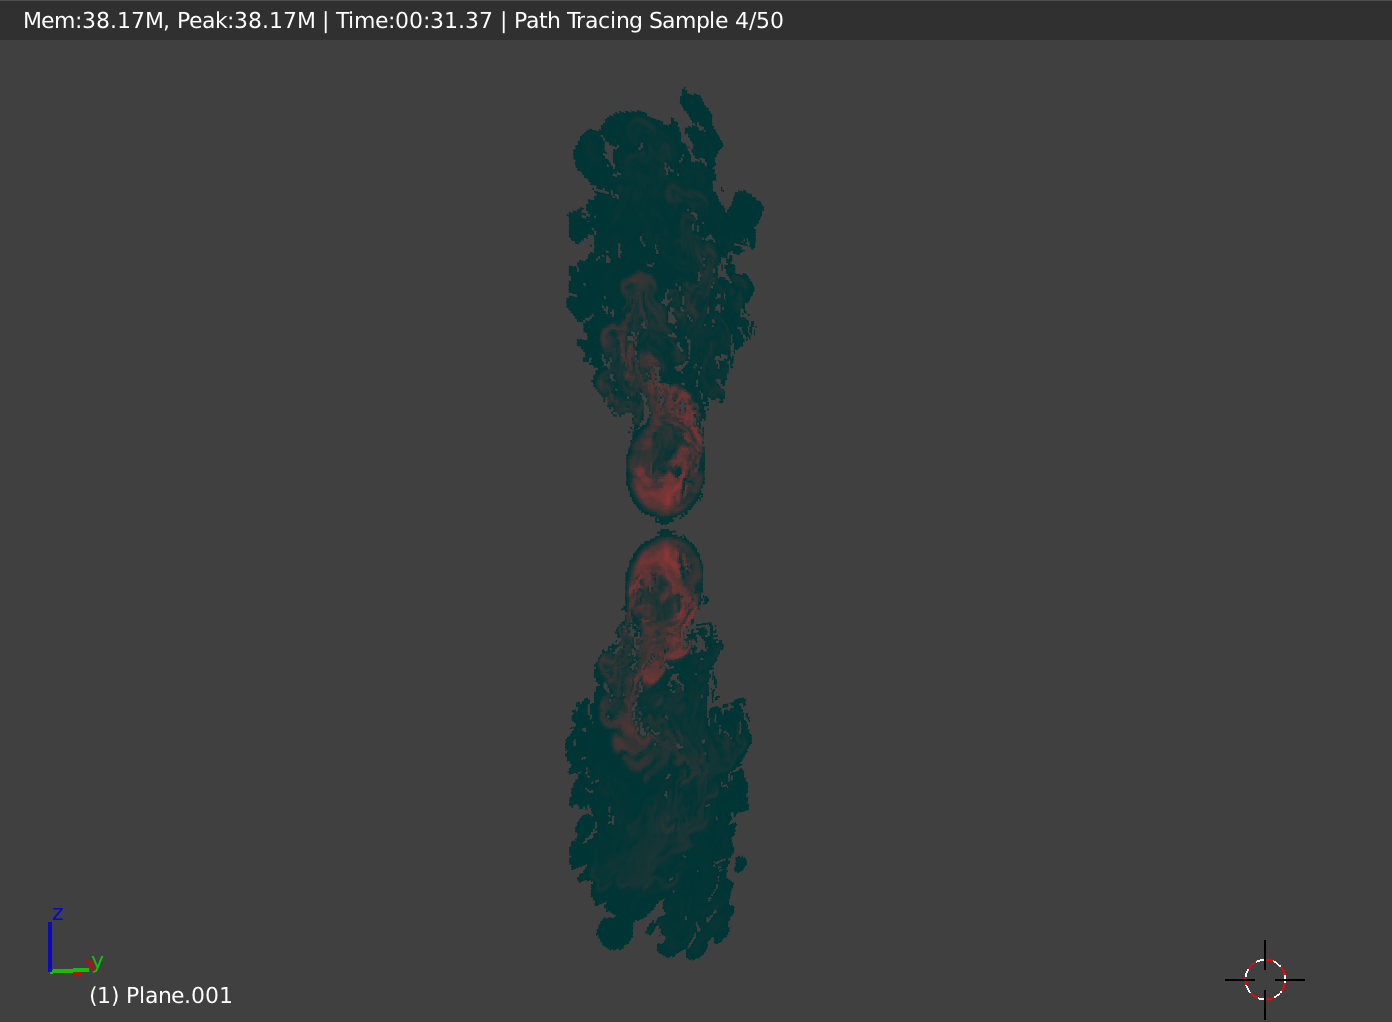
\includegraphics[width=\textwidth]{transf_upsideDown}
                \caption{Espelhamento em torno do eixo Y.}
                \label{fig:vdb_trans2}
        \end{subfigure}
        ~ %add desired spacing between images, e. g. ~, \quad, \qquad etc.
          %(or a blank line to force the subfigure onto a new line
        \begin{subfigure}{0.3\textwidth}
                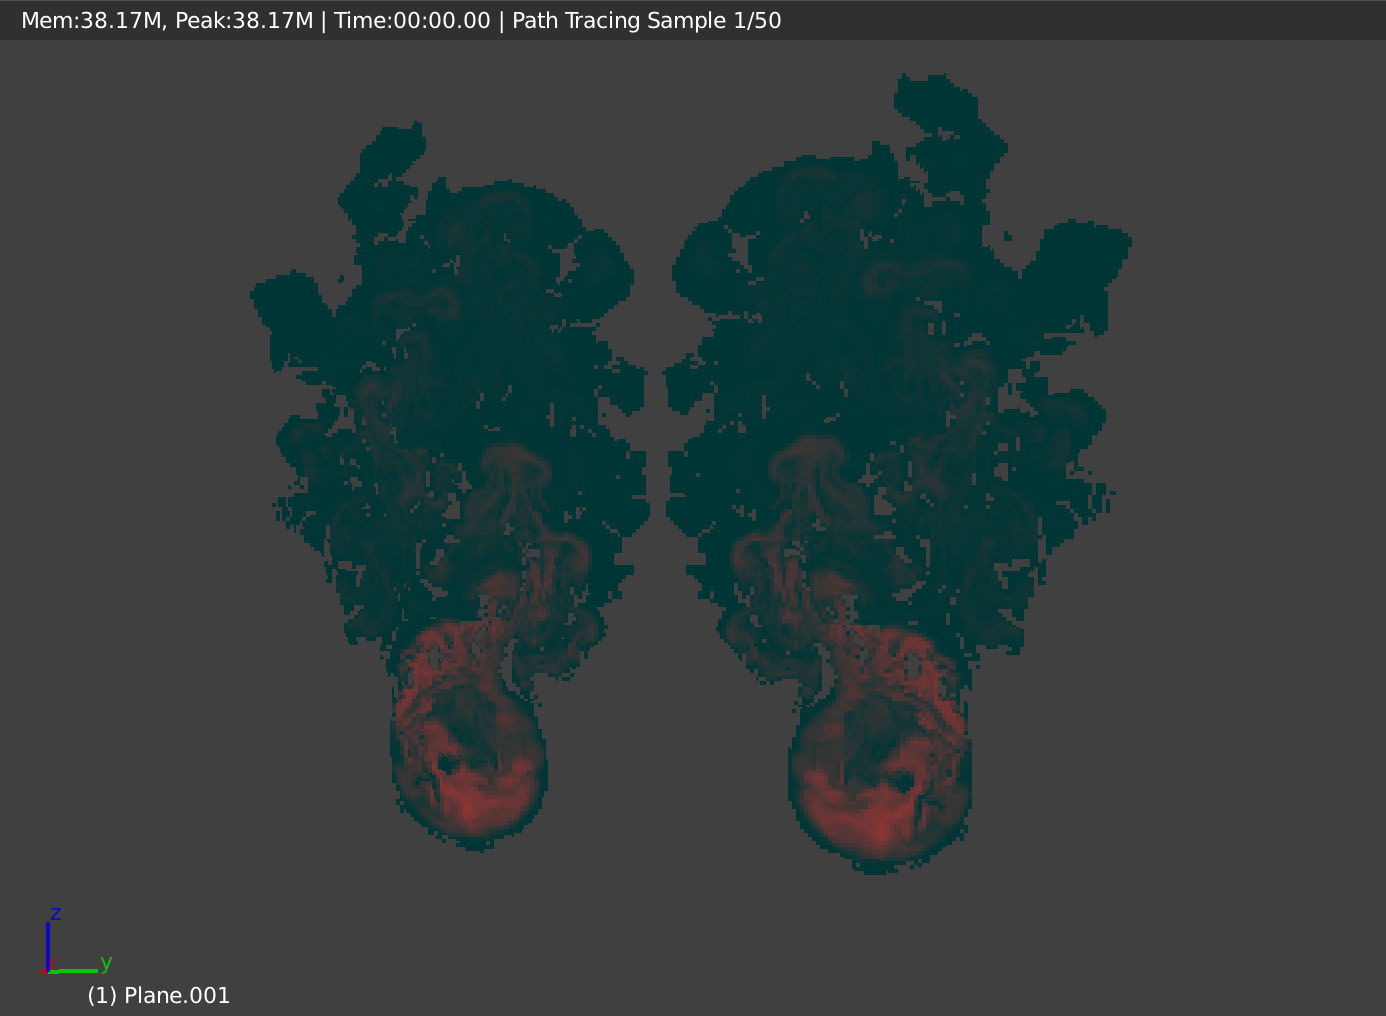
\includegraphics[width=\textwidth]{transf_Mirror}
                \caption{Espelhamento em torno do eixo Z.}
                \label{fig:vdb_trans3}
        \end{subfigure}
        \caption{A mesma fatia de volume exibida na Figura \ref{vdb_blender_interface}, com a aplicação de transformações de espelhamento.}\label{fig:vdb_trans}
\end{figure}


%figura aqui!! :-P
\begin{figure}[!htb]
\center
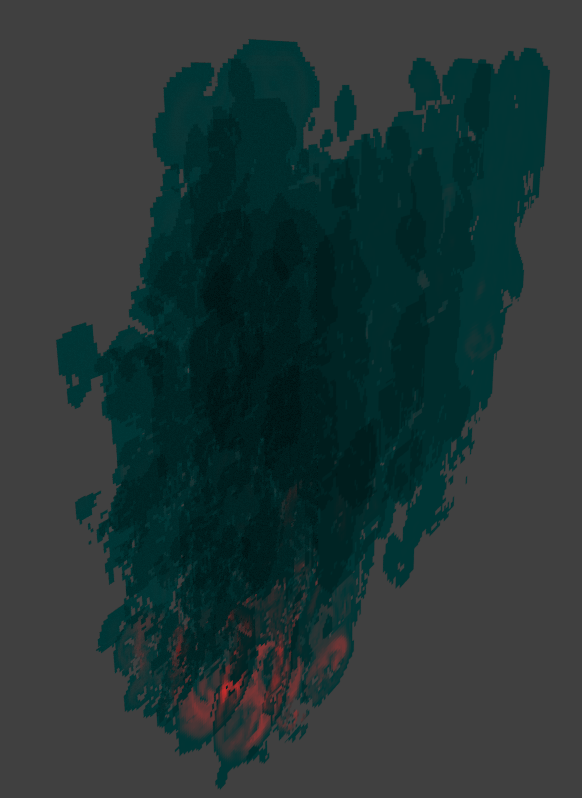
\includegraphics[width=5cm]{multiplePlanes}
\caption{Uma série de planos são posicionados próximos uns aos outros, e o volume é avaliado em cada fatia.}
\label{planes}
\end{figure}

